% !TEX root = ./main.tex


%-----------------------------------------------------------------------------
%    STARTER
%-----------------------------------------------------------------------------

\documentclass{backend/backend}
\usepackage{backend/font}
\usepackage{backend/colors}
\usepackage{backend/structure}
\usepackage{backend/informations}

%-----------------------------------------------------------------------------
%    PRESENTATION SLIDES
%-----------------------------------------------------------------------------

\begin{document}
\justifying

\begin{frame}
    \titlepage
\end{frame}

\comment{  %%%%%%%%%%%%%%%%%%%%%%%%%%%%%%%%%%%%% COMMENTARY
} %%%%%%%%%%%%%%%%%%%%%%%%%%%%%%%%%%%%% COMMENTARY


%%%%%%%%%%%%%%%%%%%%%%%%%%%%%%%%%%%%%%%%%
%
%         INTRODUCTION
%
%%%%%%%%%%%%%%%%%%%%%%%%%%%%%%%%%%%%%%%%%
\showtoctrue % active l'affichage des slides de transition
\section{Introduction}

\begin{frame}{Introduction}
    \begin{exampleblock}{HACL*}
        \textit{"\textbf{H}igh \textbf{A}ssurance \textbf{C}ryptography \textbf{L}ibrary"}\cite{HACL*}\footnote{\url{https://hacl-star.github.io/}} est une bibliothèque cryptographique, écrite en F* ("F star"), implémentant tous les algorithmes de cryptographie modernes et est prouvée mathématiquement sûre. 
        \smallbreak
        HACL* est notamment utilisé dans plusieurs systèmes de production tels que Mozilla Firefox, le noyau Linux, le VPN WireGuard...
    \end{exampleblock}
\end{frame}

\begin{frame}{Introduction - 2}
    \begin{block}{1996 : Paul C. Kocher, \textit{Timing Attacks on Implementations of Diffie-Hellman, RSA, DSS, and Other Systems} }
        Une mesure précise du temps requis par des opérations sur les clés secrètes permettrait à un attaquant de casser le cryptosystème.
    \end{block}
    2003 : \citeauthor{270176} \citetitle{270176}\\
    \pause
    2011 : \citeauthor{stillPractical} \citetitle{stillPractical}
\end{frame}

\begin{frame}[fragile]{Petit exemple}
    \begin{columns}
        \begin{column}{0.5\textwidth}
            \begin{minted}[frame=lines,framesep=2mm,baselinestretch=1.2,fontsize=\tiny,linenos, gobble=8]{C}
                bool check_pwd(msg, pwd){
                if (msg.length != pwd.length){
                    return False
                }
                for(int i = 0; i < msg.length; i++){
                    if(msg[i] != pwd[i]){
                        return False
                    }
                }
                return True
                }
            \end{minted}
            \begin{tikzpicture}[scale = 0.5, transform shape]
            % Noeuds
            \node (start) [startstop] {check\_pwd};
            \node (valid) [right of=start, xshift=9cm, green] {\huge{$\checkmark$}};
            \draw [arrow] (start) -- (valid);
            
            \node (inputs) [below of = start, yshift=0.2cm] {(msg, pwd)};
            \node (if) [process] [right of=start, xshift=2cm] {if};
            \node (not) [above of=if, red] {\huge{$\times$}};
            \node (for) [process] [right of=if,, xshift=2cm] {for};
            \node (for1) [above of=for,xshift=1cm, red] {\huge{$\times$}};
            \node (for2) [right of=for1, red] {\huge{$\times$}};
            \node (for3) [right of=for2, red] {\huge{$\times$}};

            \draw [arrow] (if) -- (not);
            \draw [arrow] (for) -- (for1);
            \draw [arrow] (for) -- (for2);
            \draw [arrow] (for) -- (for3);

            \node (t) [above of=start] {};
            \node (a) [above of=valid, xshift=-0.3cm] {};
            \draw [arrow] (t) -- node[above left] {Temps ($\mu$s)} (a.west);
            
            \end{tikzpicture}
        \end{column}
        \pause
\begin{tikzpicture}[overlay , remember picture, node distance=0.5cm]
    
    \tikzset{stop/.style={draw=red, fill=red!80, opacity=0.2}}
    
    \fill[stop] (-6.45,1.85) circle[radius=0.3cm];
    \fill[stop] (-6,0.71) circle[radius=0.3cm];

  \end{tikzpicture}
        \pause
        \begin{column}{0.5\textwidth}
            \begin{blockSimple}{Opérations influantes :}
                \begin{itemize}
                    \item Accès mémoire
                    \item Décalage/rotation de valeurs
                    \item Saut conditionnel
                    \item Division/multiplication
                \end{itemize}
            \end{blockSimple}
        \end{column}
    \end{columns}
\end{frame}


\begin{frame}{Axes de défenses contre les attaques par chronométrage}
    \begin{blockSimple}{}
        \centering
        \begin{tikzpicture}[>={Latex[length=3mm,width=2.5mm]}, link/.style={->, very thick}]

        % Nœuds avec apparition progressive
        \node[src] (src) {Source};
        \node[comp, right=18mm of src] (cmp) {Compilateur};
        \node[asm, right=18mm of cmp] (asm) {Assembleur};

        % Flèches
        \draw[link] (src) -- (cmp);
        \draw[link] (cmp) -- (asm);

        \end{tikzpicture}
    \end{blockSimple}
\end{frame}

\begin{frame}{Travail à la source}
        \centering
        \begin{tikzpicture}[scale=0.5, transform shape,>={Latex[length=3mm,width=2.5mm]}, link/.style={->, very thick}]

        % Nœuds avec apparition progressive
        \node[src] (src) {Source};
        \node[gray, right=18mm of src] (cmp) {Compilateur};
        \node[gray, right=18mm of cmp] (asm) {Assembleur};

        % Flèches
        \draw[link] (src) -- (cmp);
        \draw[link] (cmp) -- (asm);

        \end{tikzpicture}

    \vfill
    \begin{blockSimple}{Programmation en temps constant}
        \begin{columns}
            \begin{column}{0.3\textwidth}
                + Position haut niveau\\
                + Couverture d'architectures importantes
            \end{column}
            \begin{column}{0.5\textwidth}
            - Rigueur et conception particulière des actions\\
            - Identification des points de fuites
            \end{column}
        \end{columns}        
    \end{blockSimple}

    \pause
    \begin{alertblock}{2024 - \citeauthor{schneider2024breakingbadcompilersbreak}}
        \citetitle{schneider2024breakingbadcompilersbreak}
    \end{alertblock}

\end{frame}

\begin{frame}{Travail avec le compilateur}
 \centering
        \begin{tikzpicture}[scale=0.5, transform shape,>={Latex[length=3mm,width=2.5mm]}, link/.style={->, very thick}]

        % Nœuds avec apparition progressive
        \node[gray] (src) {Source};
        \node[comp, right=18mm of src] (cmp) {Compilateur};
        \node[gray, right=18mm of cmp] (asm) {Assembleur};

        % Flèches
        \draw[link] (src) -- (cmp);
        \draw[link] (cmp) -- (asm);

        \end{tikzpicture}
        \vfill
    \begin{blockSimple}{Utilisation des compilateurs}
        \begin{columns}
        \begin{column}{0.5\textwidth}
            \begin{itemize}
                \item Constantine - 2021
                \item Jasmin - 2017
                \item \alt<1>{Raccoon - 2015}{\sout{Raccoon} - 2015}
                \item CompCert - 2008 (2019)
            \end{itemize}
        \end{column}
        \begin{column}{0.5\textwidth}
          \onslide<2>{
            \begin{itemize}
            \item[-] Couverture des architectures supportée
            \item[-] Informations à transmettre
            \item[-] Spécifications ne sont plus respectées
            \end{itemize}
          }
        \end{column}
    \end{columns}
    \end{blockSimple}
\end{frame}


\begin{frame}{Travail en assembleur}
        \centering
        \begin{tikzpicture}[scale=0.5, transform shape,>={Latex[length=3mm,width=2.5mm]}, link/.style={->, very thick}]

        % Nœuds avec apparition progressive
        \node[gray] (src) {Source};
        \node[gray, right=18mm of src] (cmp) {Compilateur};
        \node[asm, right=18mm of cmp] (asm) {Assembleur};

        % Flèches
        \draw[link] (src) -- (cmp);
        \draw[link] (cmp) -- (asm);

        \end{tikzpicture}
    \vfill
        \begin{blockSimple}{Écrire en assembleur}
        \begin{columns}
            \begin{column}{0.3\textwidth}
                + Efficace\\
                + Contrôle total
            \end{column}
            \begin{column}{0.5\textwidth}
            - Spécifique à chaque processeur qui exécute\\
            - Beaucoup de connaissance spécifique au processeur ciblé\\
            - Long à mettre en place\\
            - Portabilité faible
            \end{column}
        \end{columns}        
    \end{blockSimple}

     
\end{frame}


\begin{frame}{Réalisation}
    \pause
    \begin{tikzpicture}[remember picture, overlay]
  \node[xshift = 10cm, yshift=1cm] {
    \begin{tikzpicture}[scale=0.5, transform shape,>={Latex[length=3mm,width=2.5mm]}, link/.style={->, very thick}]
\tikzstyle{arrow} = [thick,->,>=stealth, line width=1.5pt]
        % Nœuds avec apparition progressive
        \node[src] (src) {Source};
        \node[gray, right=18mm of src] (cmp) {Compilateur};
        \node[asm, right=18mm of cmp] (asm) {Assembleur};

        % Flèches
        \draw[link] (src) -- (cmp);
        \draw[link] (cmp) -- (asm);
        %\draw[->, dashed, bend left=40, >=stealth,] (src.north) to (asm.north);
        \draw [arrow, bend left, dashed, color=blue!35] (src.north) to (asm.north);

        \end{tikzpicture}
        };
    \end{tikzpicture}

    \begin{blockSimple}{Vérification de binaire}
        $\centerdot$ Approche systématisée et automatique
        $\centerdot$ Analyse correcte et complète\\
        $\centerdot$ Processus d'intégration continue
    \end{blockSimple}
    \pause
    \begin{block}{Érysichthon}
        Premier outil de vérification complète de bibliothèque cryptographique face aux attaques temporelles.            
    \end{block}


    \begin{columns}
        \begin{column}{0.4\textwidth}
            \raggedleft
            Analyse HACL* :
        \end{column}
        \begin{column}{0.7\textwidth}
            \begin{tabular}{l|c|c}
                & Prouvé & Attendu \\
                \rowcolor{lightgray}
                \hline
                (\%) Fontions sécurisées & 67,96\% & 62,39\% \\
                (\%) Fontions attaquables & 3,08\% & 27,61\% \\
                \rowcolor{lightgray}
                (\%) Analyse interrompue & 28,96\% & 0\% \\

            \end{tabular}
        \end{column}
    \end{columns}
\end{frame}



%%%%%%%%%%%%%%%%%%%%%%%%%%%%%%%%%%%%%%%%%
%
%         SUMMARY
%
%%%%%%%%%%%%%%%%%%%%%%%%%%%%%%%%%%%%%%%%%
\begin{frame}{Sommaire}
    \small
    \tableofcontents
\end{frame}

%%%%%%%%%%%%%%%%%%%%%%%%%%%%%%%%%%%%%%%%%
%
%         DEUXIEME PARTIE
%
%%%%%%%%%%%%%%%%%%%%%%%%%%%%%%%%%%%%%%%%%

\section{Outils de vérification}
\begin{frame}{Choix de l'outil}
    \begin{columns}% t = alignement en haut
    % Colonne gauche : tableau
    \column{0.6\textwidth}
    \tiny
    \begin{tabular}{lccc}
        \toprule
        \textbf{Outil} & \textbf{Cible} & \textbf{Techn.} & \textbf{Garanties} \\
        \rowcolor{lightgray}
        \alt<1,2>{ctgrind \cite{ctgrind} & Binaire & Dynamique & $\blacktriangle$}{ & & &}\\
        \alt<1>{ABPV13 \cite{ABPV13} & C & Formel & $\bullet$ }{ & & &}\\
        \rowcolor{lightgray}
        \alt<1>{VirtualCert \cite{VirtualCert} & x86 & Formel & $\bullet$ }{ & & &}\\
        \alt<1>{ct-verif \cite{ctverif} & LLVM & Formel & $\bullet$ }{ & & &}\\
        \rowcolor{lightgray}
        \alt<1>{FlowTracker \cite{FlowTracker} & LLVM & Formel & $\bullet$ }{ & & &}\\
        \alt<1>{Blazer \cite{Blazer} & Java & Formel & $\bullet$ }{ & & &}\\
        \rowcolor{lightgray}
        \alt<1>{BPT17 \cite{BPT17} & C & Symbolique & $\blacktriangle$ }{ & & &}\\
        \alt<1>{MemSan \cite{MemSan} & LLVM & Dynamique & $\blacktriangle$ }{ & & &}\\
        \rowcolor{lightgray}
        \alt<1>{Themis \cite{Themis} & Java & Formel & $\bullet$ }{ & & &}\\
        \alt<1>{COCO-CHANNEL \cite{COCOCHANNEL} & Java & Symbolique & $\bullet$ }{ & & &}\\
        \rowcolor{lightgray}
        \alt<1,2>{DATA \cite{DATA1,DATA2} & Binaire & Dynamique & $\blacktriangle$}{ & & &}\\
        \alt<1,2>{MicroWalk \cite{MicroWalk} & Binaire & Dynamique & $\blacktriangle$}{ & & &}\\
        \rowcolor{lightgray}
        \alt<1,2>{timecop \cite{timecop} & Binaire & Dynamique & $\blacktriangle$ }{ & & &}\\
        \alt<1>{SC-Eliminator \cite{SCEliminator} & LLVM & Formel & $\bullet$ }{ & & &}\\
        \rowcolor{lightgray}
        \alt<1,2>{Binsec/Rel \cite{binsecRel2019} & Binaire & Symbolique & $\blacktriangle$}{\textcolor{red}{ Binsec/Rel \cite{binsecRel2019}} & Binaire & Symbolique & $\blacktriangle$}\\
        \alt<1>{CT-WASM \cite{CTWASM} & WASM & Formel & $\bullet$ }{ & & &}\\
        \rowcolor{lightgray}
        \alt<1>{FaCT \cite{FaCT} & DSL & Formel & $\bullet$ }{ & & &}\\
        \alt<1>{haybale-pitchfork \cite{haybale-pitchfork} & LLVM & Symbolique & $\blacktriangle$ }{ & & &}\\
        \bottomrule
    \end{tabular}

    % Colonne droite : légende et titre
    \column{0.5\textwidth}
    \textbf{Liste d’outils de vérification}\\[1ex]
    Source : \cite{notThatHardCT}\\[2ex]
    \begin{scriptsize}
        
        \textbf{Cible}
        \begin{itemize}
        \item[[C, Java]] Code source
        \item[Binaire] Binaire
        \item[DSL] Surcouche de langage
        \item[Trace] Trace d'exécution
        \item[WASM] Assembleur web
    \end{itemize}
    \textbf{Techn.}
    \begin{itemize}
        \item[Formel] Programmation formelle 
        \item[[*]] type d'analyse
    \end{itemize}
    \textbf{Garanties (attaques temporelles)}\\
        $\bullet$ = Analyse correcte,$\blacktriangle$ =  Limitée
    \end{scriptsize}
    \end{columns}
\onslide<3>{}
\end{frame}


\begin{frame}{L'outil idéal}
    \begin{exampleblock}{Binsec \cite{binsecRel2019}}
       \textit{Binary Security}\footnote{\url{https://binsec.github.io/}} est une plateforme open source développée pour évaluer la sécurité des logiciels au niveau binaire. \smallbreak
       
       Il permet la recherche de vulnérabilités, la désobfuscation de logiciels malveillants et la vérification formelle de code binaire. Grâce à l'exécution symbolique, Binsec peut explorer et modéliser le comportement d'un programme pour détecter des erreurs; cette détection est réalisée en association avec des outils de fuzzing et/ou des solveurs SMT.
    \end{exampleblock}
\end{frame}


\begin{frame}[fragile]{Fonctionnement}

    \begin{blockSimple}{Détail :}
        \begin{itemize}
            \item Analyse au niveau binaire
            \item Supporte plusieurs architectures (x86\_64, ARM, PowerPC, Risc-V)
            \item Configuration automatisable
        \end{itemize}
    \end{blockSimple}
    \centering
    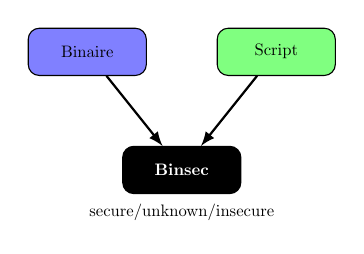
\begin{tikzpicture}[node distance=2cm, scale=0.6, transform shape]
    \tikzset{
    block/.style={
        rectangle,
        draw,
        rounded corners,
        minimum width=2.5cm,
        minimum height=1cm,
        align=center
    },
    arrow/.style={
        -latex, thick
    }
}
    \node[block,  fill=blue!50] (bin) {Binaire};
    \node[block, right of = bin, xshift=2cm, fill=green!50] (src) {Script};
    \node[block, below of = bin, yshift=-0.5cm, xshift=2cm, fill=black] (binsec) {\textcolor{white}{\textbf{Binsec}}};
    \node[below of = binsec, yshift=1.1cm] (text) {secure/unknown/insecure};

    % Flèches
    \draw[arrow] (bin) -- (binsec);
    \draw[arrow] (src) -- (binsec);
\end{tikzpicture}
    \begin{minted}{bash}
        $ binsec -sse -sse-script $(SCRIPT) -checkct $(BIN)
    \end{minted}
\end{frame}


\begin{frame}[fragile]{Usage}
    \footnotesize
    \textbf{Code :} Instructions pour trouver le mot d'un passe d'un crackme (61c8deff33c5d413767ca0ea)
    \begin{minted}[frame=lines,framesep=2mm,baselinestretch=1.2,linenos, fontsize=\tiny]{bash}
starting from core
return_address<64> := @[rsp, 8]
replace <puts>, <printf> by
  return
end
replace <__isoc99_scanf> by
  assert @[rdi, 3] = "%s"z
  len<64> := nondet         ,assume 0 < len < 50
  all_printables<1> := true
  for i<64> in 0 to len - 1 do
    @[rsi + i] := nondet as key
    all_printables := all_printables && " " <= key <= "~"
  end
  @[rsi + i] := "\x00"      ,assume all_printables
  return
end
reach <printf> such that @[rdi, 16] = "[+] Correct key!"    then print ascii stream key
cut at <printf> if @[rdi, 18] = "[-] Incorrect key!"
halt at <__stack_chk_fail>, return_address
    \end{minted}
    
        
  
    \begin{tikzpicture}[overlay , remember picture, node distance=0.5cm]
    
        \tikzset{intro/.style={rectangle, rounded corners, draw=green, fill=green!50, inner sep=0.3cm, opacity=0.2, font=\bfseries}}
        \tikzset{main/.style={rectangle, rounded corners, draw=blue, fill=blue!50, inner sep=0.3cm, opacity=0.2, font=\bfseries}}
        \tikzset{stop/.style={rectangle, rounded corners, draw=orange, fill=red!50, inner sep=0.3cm, opacity=0.2, font=\bfseries}}
        \tikzset{labelshift/.style={xshift=3cm, yshift=0.5cm}}
        
        \onslide<4->{
        \node[stop, fit={(0.3,0.2) (12.74,1.3)}, label={[labelshift]center:Stop}]{};}
        \onslide<3->{\node[main,  fit={(0.3,1.9) (12.74,4.5)}, label={[labelshift]center:Stubs}]{};}
        \onslide<3->{\node[main,  fit={(0.3,5.1) (12.74,5.6)}, label={[labelshift,yshift=-0.5cm]center:Stubs}]{};}        
        \onslide<2->{\node[intro, fit={(0.3,6.2) (12.74,6.2)}, label={[labelshift, yshift=-0.5cm]center:Chargement des données}]{};}

  \end{tikzpicture}
\end{frame}
    
\begin{frame}[fragile]{Retour de Binsec}
    \begin{minted}[frame=lines,framesep=2mm,baselinestretch=1.2,linenos, fontsize=\tiny]{bash}
$ binsec -sse -sse-script crackme.ini -sse-depth 10000 core.snapshot
[sse:result] Path 22 reached address 0x7ffff7e115b0 (<printf>) (0 to go)
[sse:result] Ascii stream key : "34407373373234353336"
[sse:info] SMT queries
             Preprocessing simplifications      Satisfiability queries
               total          20894               total          80
               true           5243                sat            41
               false          10923               unsat          39
               constant enum  4728                unknown        0
                                                  time           0.39
                                                  average        0.00
           Exploration
             total paths                      22
             completed/cut paths              19
             pending paths                    3
             stale paths                      0
             failed assertions                0
             branching points                 20931
             max path depth                   7212
             visited instructions (unrolled)  143268
             visited instructions (static)    3720
    \end{minted}

    \begin{tikzpicture}[overlay , remember picture, node distance=0.5cm]
    
        \tikzset{command/.style={rectangle, rounded corners, draw=orange, fill=orange, inner sep=0.3cm, opacity=0.2, font=\bfseries}}
        \tikzset{result/.style={rectangle, rounded corners, draw=blue, fill=blue!50, inner sep=0.3cm, opacity=0.2, font=\bfseries}}
        \tikzset{key/.style={rectangle, rounded corners, draw=red, fill=red!50, inner sep=0.3cm, opacity=0.2, font=\bfseries}}
        \tikzset{labelshift/.style={xshift=3cm, yshift=0.5cm}}
        
        \onslide<2->{\node[result,  fit={(0.3,0.1) (12.74,6.1)}, label={[labelshift]center:Résultats}]{};}
        \onslide<2->{\node[command, fit={(0.3,6.8) (12.74,6.8)}, label={[labelshift]center:Commande}]{};}
        \onslide<3->{\node[key,     fit={(3.9,6) (6,6)}, label={[xshift=1.3cm]center:Clé}]{};}
        

  \end{tikzpicture}
\end{frame}


\section{Automatisme}
\subsection{Étude sur cas simple}
\begin{frame}[fragile]{Étude sur cas simple}
\begin{columns}

  % Colonne de gauche : code C
  \column{0.55\textwidth}
  \textbf{Codes :} Test de la fonction \textit{bn\_cmovznz4}
    
  \begin{minted}[frame=lines,framesep=2mm,baselinestretch=1.2,linenos,fontsize=\scriptsize]{C}
#include <stdlib.h>
#include <stdint.h>
#include "Hacl_P256.h"

#define SIZE 4
uint64_t cin;
uint64_t x[SIZE]; uint64_t y[SIZE]; uint64_t r[SIZE];

int main(){
  bn_cmovznz4(r, cin, x, y);
}
  \end{minted}

%   \onslide<2>{
%     \begin{tikzpicture}[overlay, remember picture, node distance=0.5cm]
%       \tikzset{stop/.style={rectangle, rounded corners, draw=red, fill=red!80, inner sep=0.3cm, opacity=0.2}}
%       \node[stop, fit={(0.3,2.3) (12.74,3.5)}]{};
%     \end{tikzpicture}
%   }

  % Colonne de droite : script d’analyse
  \column{0.45\textwidth}
  \textbf{Codes :} Script Binsec associé
    
  \begin{minted}[frame=lines,framesep=2mm,baselinestretch=1.2,linenos,fontsize=\scriptsize]{bash}
load sections .plt, .text, .rodata, .data, .got, .got.plt, .bss from file

secret global  r, cin, y, x

starting from <main>

with concrete stack pointer
halt at  0x0000000000000464
explore all

  \end{minted}

\end{columns}
\end{frame}

\begin{frame}{Analyse de compilateur}
    
    \textbf{Table :} Résultats d'analyse Binsec pour plusieurs compilateurs vers ARM
    \begin{center}
    \resizebox{\textwidth}{!}{%
    \begin{tabular}{|c|ccccccc|ccccccc|}
        \hline
        \rowcolor{blue!10}
        \cellcolor{inria-2024-gris-bleu!20}\textbf{opt}\textbackslash\textbf{fonction - architecture} 
            & \multicolumn{7}{|c|}{\textbf{cmovznz4 - 64b}}
            & \multicolumn{7}{|c|}{\textbf{cmovznz4 - 32b}} \\
        \hline
        \rowcolor{blue!30}
        Compilateur (Clang+LLVM par défaut)  & gcc 15.1.0 & clang 14.0.6 & 15.0.6 & 16.0.4 & 17.0.6 & 18.1.8 & 19.1.7 
        & gcc 15.1.0 & clang 14.0.6 & 15.0.6 & 16.0.4 & 17.0.6 & 18.1.8 & 19.1.7 \\
        \hline
        \rowcolor{orange!30!red!50}
        \textbf{-O0} & \cellcolor{orange!60}\textasciitilde & \cellcolor{green!60}\checkmark & \cellcolor{green!60}\checkmark & \cellcolor{green!60}\checkmark & \cellcolor{green!60}\checkmark & \cellcolor{green!60}\checkmark 
        & \cellcolor{red!60}$\times$ 
        & \cellcolor{orange!60}\textasciitilde & \cellcolor{green!60}\checkmark & \cellcolor{green!60}\checkmark & \cellcolor{green!60}\checkmark & \cellcolor{green!60}\checkmark & \cellcolor{green!60}\checkmark 
        & \cellcolor{red!60}$\times$  \\
        \hline
        \rowcolor{orange!30!red!50}
        \textbf{-O1} & \cellcolor{green!60}\checkmark & \cellcolor{green!60}\checkmark & \cellcolor{green!60}\checkmark & 
        \cellcolor{green!60}\checkmark & \cellcolor{green!60}\checkmark & \cellcolor{green!60}\checkmark & \cellcolor{red!60}$\times$
        & \cellcolor{green!60}\checkmark & \cellcolor{green!60}\checkmark & \cellcolor{green!60}\checkmark & 
        \cellcolor{green!60}\checkmark & \cellcolor{green!60}\checkmark & \cellcolor{green!60}\checkmark & \cellcolor{red!60}$\times$ \\
        \hline
        \rowcolor{orange!30!red!50}
        \textbf{-O2} & \cellcolor{green!60}\checkmark & \cellcolor{green!60}\checkmark & \cellcolor{green!60}\checkmark & 
        \cellcolor{green!60}\checkmark & \cellcolor{green!60}\checkmark & \cellcolor{green!60}\checkmark & \cellcolor{red!60}$\times$
        & \cellcolor{green!60}\checkmark & \cellcolor{green!60}\checkmark & \cellcolor{green!60}\checkmark & 
        \cellcolor{green!60}\checkmark & \cellcolor{green!60}\checkmark & \cellcolor{green!60}\checkmark & \cellcolor{red!60}$\times$  \\
        \hline
        \rowcolor{orange!30!red!50}
        \textbf{-O3} & \cellcolor{green!60}\checkmark & \cellcolor{green!60}\checkmark & \cellcolor{green!60}\checkmark & 
        \cellcolor{green!60}\checkmark & \cellcolor{green!60}\checkmark & \cellcolor{green!60}\checkmark & \cellcolor{red!60}$\times$
        & \cellcolor{green!60}\checkmark & \cellcolor{green!60}\checkmark & \cellcolor{green!60}\checkmark & 
        \cellcolor{green!60}\checkmark & \cellcolor{green!60}\checkmark & \cellcolor{green!60}\checkmark & \cellcolor{red!60}$\times$  \\
        \hline
        \rowcolor{orange!30!red!50}
        \textbf{-Os} & \cellcolor{green!60}\checkmark & \cellcolor{green!60}\checkmark & \cellcolor{green!60}\checkmark & 
        \cellcolor{green!60}\checkmark & \cellcolor{green!60}\checkmark & \cellcolor{green!60}\checkmark & \cellcolor{red!60}$\times$
        & \cellcolor{green!60}\checkmark & \cellcolor{green!60}\checkmark & \cellcolor{green!60}\checkmark & 
        \cellcolor{green!60}\checkmark & \cellcolor{green!60}\checkmark & \cellcolor{green!60}\checkmark & \cellcolor{red!60}$\times$  \\
        \hline
        \rowcolor{orange!30!red!50}
        \textbf{-Oz} & \cellcolor{green!60}\checkmark & \cellcolor{green!60}\checkmark & \cellcolor{green!60}\checkmark & 
        \cellcolor{green!60}\checkmark & \cellcolor{green!60}\checkmark & \cellcolor{green!60}\checkmark & \cellcolor{red!60}$\times$
        & \cellcolor{green!60}\checkmark & \cellcolor{green!60}\checkmark & \cellcolor{green!60}\checkmark & 
        \cellcolor{green!60}\checkmark & \cellcolor{green!60}\checkmark & \cellcolor{green!60}\checkmark & \cellcolor{red!60}$\times$  \\
        \hline
    \end{tabular}}
    \end{center}
    \raggedleft
    \small{
        \checkmark : \textit{binary secure} ; 
        \textasciitilde : \textit{binary unknown} ; 
        $\times$ : \textit{binary insecure}
    }
\end{frame}


\subsection{Contraintes et identification des limitations}
\begin{frame}{Points d'attention}
    \begin{columns}
        \begin{column}{0.4\textwidth}
            \begin{blockSimple}{Dépendances des informations}
                \onslide<2>{\begin{itemize}
                    \item Variables secrètes
                    \item Test correct
                \end{itemize}}
            \end{blockSimple}
        \end{column}
        
        \begin{column}{0.5\textwidth}
            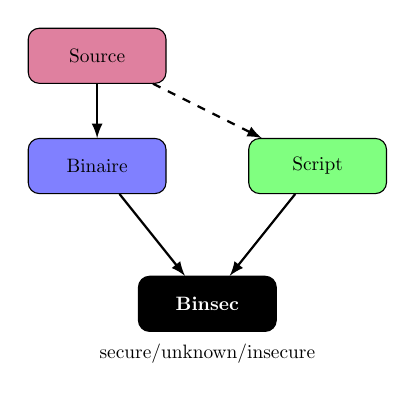
\begin{tikzpicture}[node distance=2cm, scale=0.7, transform shape]
                \tikzset{ block/.style={rectangle,draw,rounded corners,minimum width=2.5cm,minimum height=1cm,align=center},
                        arrow/.style={-latex, thick}}
                \node[block,  fill=blue!50] (bin) {Binaire};
                \node[block, right of = bin, xshift=2cm, fill=green!50] (src) {Script};
                \node[block, below of = bin, yshift=-0.5cm, xshift=2cm, fill=black] (binsec) {\textcolor{white}{\textbf{Binsec}}};
                \node[below of = binsec, yshift=1.1cm] (text) {secure/unknown/insecure};
                
                % Flèches
                \draw[arrow] (bin) -- (binsec);
                \draw[arrow] (src) -- (binsec);

                \node[block,  fill=purple!50, above of = bin] (source) {Source};
                \draw[arrow] (source) -- (bin);
                \draw[arrow, dashed] (source) -- (src);
                
            \end{tikzpicture}
        \end{column}
    \end{columns}
    
\end{frame}


\begin{frame}{Cahier des charges}
\begin{columns}
    \column{0.5\textwidth}
    \begin{blockSimple}{Objectifs du futur outil}
        \begin{itemize}
            \item Petits fichiers binaire
            \item Analyse correcte
            \item Analyse complète de la bibliothèque
            \item Automatique
            \item Couverture [\textit{architectures, compilateurs}] 
        \end{itemize}
    \end{blockSimple}
    \pause
    \column{0.5\textwidth}
    \textbf{Figure :} Flot de travail de l'outil
    \smallbreak
    \begin{tikzpicture}[ scale=0.7, transform shape]
        \begin{scope}[shift={([yshift=-2.3cm, xshift=-1cm]current page.north)}]
    % Styles
    \tikzstyle{startstop} = [rectangle, rounded corners, minimum width=2cm, minimum height=1cm, text centered, draw=black, fill=green!30]
    \tikzstyle{process} = [rectangle, minimum width=2cm, minimum height=1cm, text centered, draw=black, fill=orange!30]
    \tikzstyle{arrow} = [thick,->,>=stealth]
    \tikzset{zone1/.style={rectangle, rounded corners, draw=red, dashed, fill=red!10, inner sep=0.3cm}}
    \tikzset{zone2/.style={rectangle, rounded corners, draw=blue, dashed, fill=blue!10, inner sep=0.3cm, opacity = 0.5}}
    \tikzset{zone3/.style={rectangle, rounded corners, draw=green, dashed, fill=green!10, inner sep=0.3cm}}
    
    % Noeuds
    \node (hacl) [startstop] {HACL*};
    \node (c) [below of=hacl] {Fonction};
    \node (ini) [below of=c] {.ini};
    \node (test) [below of=c, xshift=-2cm] {-test.c};
    \node (compilateur) [process, below of=test] {Compilateur};
    \node (exe) [below of=compilateur] {-test.exe};
    \node (blanc) [below of=c] {};
    \node (blanc1) [below of=blanc] {};
    \node (blanc2) [below of=blanc1] {};
    \node (binsec) [startstop, below of=blanc2] {Binsec};
    
    % Flèches
    \draw [arrow] (hacl) -- (c);
    \draw [arrow] (c) -- (ini);
    \draw [arrow] (c) -- (test);
    \draw [arrow] (test) -- (compilateur);
    \draw [arrow] (compilateur) -- (exe);
    \draw [arrow] (exe) -- (binsec);
    \draw [arrow] (ini) -- (binsec);

    % Zones
    \begin{scope}[on background layer]
        \node [zone1, fit=(c) (ini) (test) ] {};
        \node [zone2, fit=(ini) (binsec)] {};
        \node [zone3, fit=(compilateur) (exe)] {};
    \end{scope}
    \end{scope}
\node[anchor=north west] at (ini.north east) {
    \begin{tikzpicture}[font=\small]
    \node[rectangle, draw=black, fill=white, rounded corners, inner sep=2mm] {
        \begin{tabular}{l}
        \textbf{Légende :} \\
        \textcolor{red}{\rule{0.5cm}{0.3cm}} Difficile \\
        \textcolor{blue}{\rule{0.5cm}{0.3cm}} Relativement simple \\
        \textcolor{green}{\rule{0.5cm}{0.3cm}} Simple
        \end{tabular}
    };
    \end{tikzpicture}
};
    \end{tikzpicture}
\end{columns}
\end{frame}

\begin{frame}{Adaptation architecturale}
    \begin{tikzpicture}[remember picture, overlay]
    \begin{scope}[shift={([yshift=-2.3cm, xshift=-3cm]current page.north)}]
    % Styles
    \tikzstyle{startstop} = [rectangle, rounded corners, minimum width=2cm, minimum height=1cm, text centered, draw=black, fill=green!30]
    \tikzstyle{process} = [rectangle, minimum width=2cm, minimum height=1cm, text centered, draw=black, fill=orange!30]
    \tikzstyle{arrow} = [thick,->,>=stealth]
    \tikzset{zone1/.style={rectangle, rounded corners, draw=red, dashed, fill=red!10, inner sep=0.3cm}}
    \tikzset{zone2/.style={rectangle, rounded corners, draw=blue, dashed, fill=blue!10, inner sep=0.3cm, opacity = 0.7}}
    \tikzset{zone22/.style={rectangle, rounded corners, draw=none, fill=blue!10, inner sep=0.3cm}}
    \tikzset{zone3/.style={rectangle, rounded corners, draw=green, dashed, fill=green!10, inner sep=0.3cm}}
    
    % Noeuds
    \node (hacl) [startstop] {HACL*};
    \node (c) [below of=hacl] {Fonction};
    \node (ini) [below of=c, xshift=2cm] {.ini};
    \node (test) [below of=c, xshift=-2cm] {-test.c};
    \node (script) [below of=c] {.script};
    \node (compilateur) [process, below of=test] {Compilateur};
    \node (exe) [below of=compilateur] {-test.exe};
    \node (blanc1) [below of=script] {};
    \node (blanc2) [below of=blanc1] {};
    \node (gdb) [process, below of=blanc2] {GDB};
    \node (snap) [right of=gdb, xshift=2cm] {.snapshot};
    \node (binsec) [startstop, right of=snap, xshift=1.5cm] {Binsec};
    
    % Flèches
    \draw [arrow] (hacl) -- (c);
    \draw [arrow] (c) -- (ini);
    \draw [arrow] (c) -- (test);
    \draw [arrow] (c) -- (script);
    \draw [arrow] (test) -- (compilateur);
    \draw [arrow] (compilateur) -- (exe);
    \draw [arrow] (exe) -- (gdb);
    \draw [arrow] (script) -- (gdb);
    \draw [arrow] (gdb) -- (snap);
    \draw [arrow] (snap) -- (binsec);
    \draw [arrow] (ini) -- (binsec);

    % Zones
    \begin{scope}[on background layer]
        \node [zone1, fit=(c) (ini) (test) (script)] {};
        \node [zone2, fit=(script) (gdb)] {};
              \node [zone2, fit=(gdb) (snap) (binsec)] {};
              \draw [zone22]
              ([xshift=-10pt, yshift=10pt]gdb.north west) --
              ([xshift=10pt, yshift=10pt]gdb.north east) -- 
              ([xshift=10pt, yshift=-9pt]gdb.south east) -- 
              ([xshift=1pt, yshift=-1pt]gdb.south west) --
              cycle;  
    \node [zone3, fit=(compilateur) (exe)] {};
    \end{scope}
\end{scope}
    \node[anchor=north east] at ([xshift=-5mm,yshift=-3cm]current page.north east) {
    \begin{tikzpicture}[font=\small]
    \node[rectangle, draw=black, fill=white, rounded corners, inner sep=2mm] {
        \begin{tabular}{l}
        \textbf{Légende :} \\
        \textcolor{red}{\rule{0.5cm}{0.3cm}} Difficile \\
        \textcolor{blue}{\rule{0.5cm}{0.3cm}} Relativement simple \\
        \textcolor{green}{\rule{0.5cm}{0.3cm}} Simple
        \end{tabular}
    };
\end{tikzpicture}
};
\end{tikzpicture}
\end{frame}

\section{Érysichthon}
\subsection{Conception générale}

\begin{frame}{Construction en modules}
    \begin{center}
        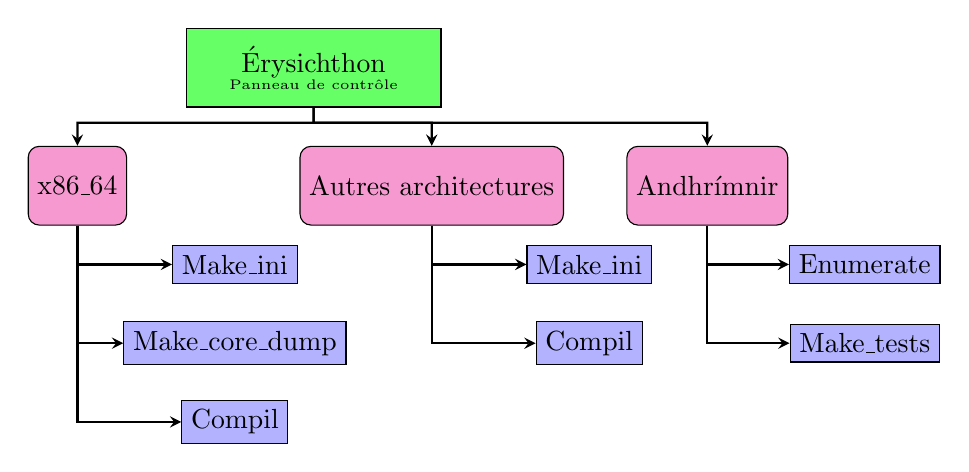
\begin{tikzpicture}[auto]

    % Styles
    \tikzstyle{startstop} = [rectangle, minimum width=2cm, minimum height=1cm, text centered, draw=black, fill=green!60]
    \tikzstyle{process} = [rectangle, rounded corners,minimum width=1cm, minimum height=1cm, text centered, draw=black, fill=magenta!40]
     \tikzstyle{process2} = [rectangle, minimum width=0.8cm, minimum height=0.3cm, text centered, draw=black, fill=blue!30]
    \tikzstyle{arrow} = [thick,->,>=stealth]
    
    % Noeuds
    \node (control) [startstop] {\parbox{3cm}{\centering Érysichthon \\ \tiny{Panneau de contrôle}}};
    \node (x86) [process, below of=control, xshift= -3cm, yshift=-0.5cm] {x86\_64};
    \node (x86-ini) [process2, below of=x86, xshift = 2cm] {Make\_ini};
    \node (x86-dump) [process2, below of=x86-ini] {Make\_core\_dump};
    \node (x86-compil) [process2, below of=x86-dump] {Compil};

    \node (arm) [process, below of=control, xshift = 1.5cm, , yshift=-0.5cm] {Autres architectures};
    \node (arm-ini) [process2, below of=arm, xshift=2cm] {Make\_ini};
    \node (arm-compil) [process2, below of=arm-ini] {Compil};

    \node (test) [process, below of=control, xshift = 5cm, , yshift=-0.5cm] {Andhrímnir};
    \node (enum) [process2, below of=test, xshift=2cm] {Enumerate};
    \node (exe) [process2, below of=enum] {Make\_tests};

    % Flèches
    \draw [arrow] (control) -- ++(0,-0.7) -- ++(-3,0) -- (x86.north);
    \draw [arrow] (control) -- ++(0,-0.7) -- ++(1.5,0) -- (arm.north);
    \draw [arrow] (control) -- ++(0,-0.7) -- ++(5,0) -- (test.north);
    \draw [arrow] (x86) -- ++(0,-1) -- (x86-ini);
    \draw [arrow] (x86) -- ++(0,-2) -- (x86-dump);
    \draw [arrow] (x86) -- ++(0,-3) -- (x86-compil);
    \draw [arrow] (arm) -- ++(0,-1) -- (arm-ini);
    \draw [arrow] (arm) -- ++(0,-2) -- (arm-compil);
    \draw [arrow] (test) -- ++(0,-1) -- (enum);
    \draw [arrow] (test) -- ++(0,-2) -- (exe);
    
    \end{tikzpicture}
    \end{center}
\end{frame}


\subsection{Andhrímnir}

\begin{frame}{Andhrímnir - 1}
    \begin{columns}
        \begin{column}{0.5\textwidth}
            \begin{blockSimple}{Module indépendant}
                \begin{itemize}
                    \item Réalise des tests automatiquement
                    \item Réalise des tests corrects
                \end{itemize}
            \end{blockSimple}
            \pause
            \begin{blockSimple}{Module adapté}
                \begin{itemize}
                    \item Optimisation pour HACL*
                    \item Communications avec Érysichthon
                    \item Adaptées pour l'analyse symbolique avec Binsec
                \end{itemize}
            \end{blockSimple}
        \end{column}
        \pause
        \begin{column}{0.45\textwidth}
            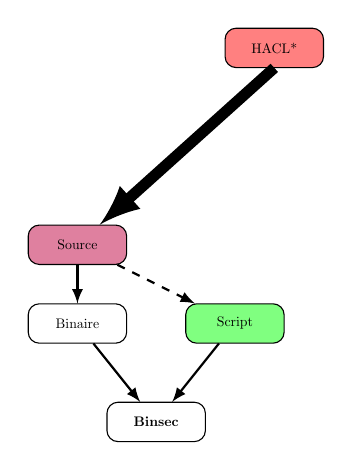
\begin{tikzpicture}[node distance=2cm, scale=0.5, transform shape]
                \tikzset{ block/.style={rectangle,draw,rounded corners,minimum width=2.5cm,minimum height=1cm,align=center},
                        arrow/.style={-latex, thick}}
                \node[block,] (bin) {Binaire};
                \node[block,  fill=purple!50, above of = bin] (source) {Source};
                \node[block, right of = bin, xshift=2cm, fill=green!50] (src) {Script};
                \node[block, below of = bin, yshift=-0.5cm, xshift=2cm] (binsec) {\textbf{Binsec}};
        
                % Flèches
                \draw[arrow] (bin) -- (binsec);
                \draw[arrow] (src) -- (binsec);
                \draw[arrow] (source) -- (bin);
                \draw[arrow, dashed] (source) -- (src);

                \node[above of = source, xshift=5cm] (json) {};
                \node[block,  fill=red!50, above of = json, yshift=1cm] (hacl) {HACL*};
                \draw[arrow,  line width=4pt] (hacl.south) -- (source);
            \end{tikzpicture}
        \end{column}
    \end{columns}
\end{frame}

\begin{frame}{Andhrímnir - 2}
    \begin{tikzpicture}[scale = 0.7, transform shape]
    % Définition des styles pour les boîtes et flèches
    \tikzset{
      box1/.style={rectangle, draw=black, fill=cyan!30, thick, rounded corners, minimum width=2.5cm, minimum height=1cm, align=center},
      box2/.style={rectangle, draw=black, fill=orange!30, thick, rounded corners, minimum width=2.5cm, minimum height=1cm, align=center},
      box3/.style={rectangle, draw=black, fill=yellow!30, thick, rounded corners, minimum width=2.5cm, minimum height=1cm, align=center},
      box4/.style={rectangle, draw=black, fill=green!30, thick, rounded corners, minimum width=2.5cm, minimum height=1cm, align=center},
      box5/.style={rectangle, draw=black, fill=blue!30, thick, rounded corners, minimum width=2.5cm, minimum height=1cm, align=center},
      box6/.style={rectangle, draw=black, fill=magenta!30, thick, rounded corners, minimum width=2.5cm, minimum height=1cm, align=center},
      box65/.style={rectangle, draw=black, fill=magenta!60, thick, rounded corners, minimum width=1.5cm, minimum height=0.6cm, align=center},
      box7/.style={rectangle, draw=black, fill=red!30, thick, rounded corners, minimum width=2.5cm, minimum height=1cm, align=center},
      box8/.style={rectangle, draw=black, fill=blue!45, thick, rounded corners, minimum width=2.5cm, minimum height=1cm, align=center},
      arrow1/.style={->, thick, color=cyan!70!black},
      arrow2/.style={->, thick, color=orange!80!black},
      arrow3/.style={->, thick, color=yellow!80!black},
      arrow4/.style={->, thick, color=green!80!black},
      arrow5/.style={->, thick, color=blue!80!black},
      arrow6/.style={->, thick, color=magenta!80!black},
      arrow7/.style={->, thick, color=red!80!black},
      arrow8/.style={->, thick, color=gray!80!black}
      }
      \tikzset{zone1/.style={rectangle, rounded corners, draw=blue, dashed, fill=blue!10, inner sep=0.5cm, text width=3cm}}

    % Noeuds principaux (ligne du haut)
    \node[] (build_test) at (0,0) {};
    \node[box2, below of=build_test] (parse_h) {Lecture du projet C};
    \node[box3, right=1cm of parse_h] (read_json) {Vérification mémoire (json)};
    \node[box4, right=1cm of read_json] (build_local_json) {Accumulation d'informations};

    % Ligne du bas (génération du .c)
    \node[box5, below=1cm of build_local_json] (build_intro) {Gen. introduction};
    \node[box6, left=1cm of build_intro] (build_def) {Gen. déclaration};
    \node[box7, left=1cm of build_def] (add_main) {Gen. main};
    \node[box8, left=1cm of add_main] (fichier_c) {fichier .c};

    % Flèches horizontales principales
    \draw[arrow2] (parse_h) -- (read_json);
    \draw[arrow3] (read_json) -- (build_local_json);
    \draw[arrow4] (build_local_json) -- (build_intro);
    \draw[arrow5] (build_intro) -- (build_def);
    \draw[arrow6] (build_def) -- (add_main);
    \draw[arrow7] (add_main) -- (fichier_c);

    % Branche auxiliaire depuis build introduction
    \node[box5, left of = build_intro, yshift=-1cm] (detect_aux) {Détection appel auxiliaire};
    % Ajout de deux barres obliques sur la flèche build_intro -> build_def
    \draw[thick] ($(build_intro)!0.5!(build_def) + (0,0.3)$) -- ($(build_intro)!0.5!(build_def) + (0,-0.54)$);
    \draw[thick] ($(build_intro)!0.55!(build_def) + (0,0.3)$) -- ($(build_intro)!0.55!(build_def) + (0,-0.54)$);


    \node[box3, left=1cm of detect_aux, yshift=-2cm] (test_exist) {test si fichier existe};
    \draw[arrow5] (detect_aux) -- (test_exist);

    % Oui -> Collage -> build definition
    \node[box4, above of = test_exist, yshift=0.5cm] (collage) {\footnotesize{Collage}};
    \draw[->, thick, color=green!80!black] (test_exist) -- node[left, font=\scriptsize] {Oui} (collage);
    \draw[arrow6] (collage) -- (build_def);

    % Non -> Stocker dans liste_temporisée
    \node[box2, left=0.8cm of test_exist, yshift=-0.8cm] (liste_temp) {Stocker dans liste\_temporisée};
    \draw[arrow7] (test_exist) -- node[above,font=\scriptsize] {Non} (liste_temp.east);

    \draw [arrow5, dashed] (liste_temp.east) to[out=-30, in=-30] node[black, below, yshift=-0.5cm] {\textit{Recommence le procédé}} (build_intro.east);

    \begin{scope}[on background layer]
      \node (zoneNode) [zone1, fit=(parse_h) (read_json) (build_local_json) (build_intro) (build_def) (add_main) (fichier_c) (test_exist) (liste_temp) (collage) (detect_aux) (build_test)] {};
        \node (title) [anchor=north west] at (zoneNode.north west) {\parbox{3.5cm}{\centering \Huge{\textbf{Andhrímnir}}\\\scriptsize{\textit{Génère les tests}}}};
    \end{scope}
  \end{tikzpicture}
\end{frame} 


\begin{frame}[fragile]{Exemple de test}
    \textbf{Code :}Test de la fonction Hacl\_EC\_K256\_felem\_sqr
  \begin{minted}[fontsize=\scriptsize]{c}
// Made by
// ANDHRÍMNIR - 0.3.0
// 09-07-2025
//

#include <stdlib.h>
#include "Hacl_EC_K256.h"

#define BUFFER_SIZE 5
uint64_t a[BUFFER_SIZE];
uint64_t out[BUFFER_SIZE];


int main (int argc, char *argv[]){
Hacl_EC_K256_felem_sqr(a, out);
  exit(0);
}   
  \end{minted}
\onslide<2>{
  \begin{tikzpicture}[overlay , remember picture, node distance=0.5cm]
    
    \tikzset{intro/.style={rectangle, rounded corners, draw=green, fill=green!50, inner sep=0.3cm, opacity=0.2, font=\bfseries}}
    \tikzset{definition/.style={rectangle, rounded corners, draw=blue, fill=blue!50, inner sep=0.3cm, opacity=0.2, font=\bfseries}}
    \tikzset{main/.style={rectangle, rounded corners, draw=orange, fill=orange!50, inner sep=0.3cm, opacity=0.2, font=\bfseries}}
    \tikzset{labelshift/.style={xshift=3cm, yshift=0.5cm}}

    \node[intro, fit={(0.3,4.1) (12.74,5.9)}, label={[labelshift]center:Phase introductive : 8 lignes}]{};
    \node[definition, fit={(0.3,2.3) (12.74,3.5)}, label={[labelshift]center:Phase déclarative}]{};
    \node[main, fit={(0.3,0.8) (12.74,1.7)}, label={[labelshift]center:Phase principale}]{};

  \end{tikzpicture}
}
\end{frame}



\section{Résultats}
\begin{frame}{Premières passes}
    \begin{center}
        \textbf{Graphe :} Résultats d'Érysichthon en x86\_64, \texttt{gcc 12.2.0}
    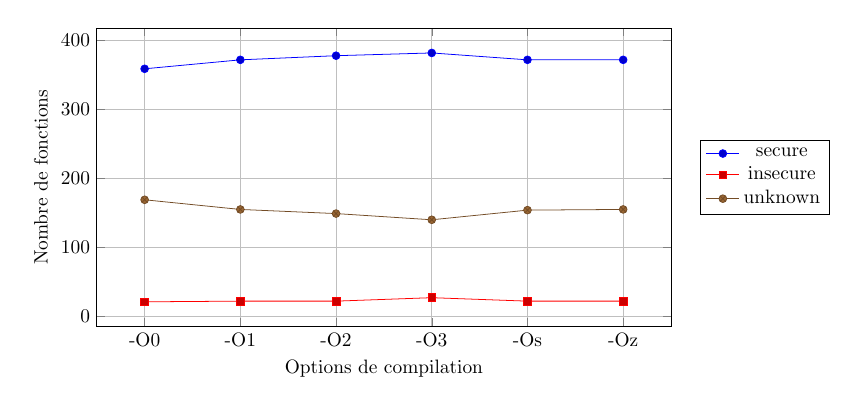
\begin{tikzpicture}[scale = 0.7, transform shape]
      \begin{axis}[
        xlabel={Options de compilation},
        ylabel={Nombre de fonctions},
        legend style={at={(0.5,-0.15)},anchor=north,legend columns=-1},
        grid=both,
        xtick={0,1,2,3,4,5},
        xticklabels={-O0, -O1, -O2, -O3, -Os, -Oz},
        width=12cm, height=7cm,
        legend style={at={(1.05,0.5)}, anchor=west},
        legend columns=1
      ]

        \addplot coordinates {(0,359) (1,372) (2,378) (3,382) (4,372) (5,372)};
        \addlegendentry{secure}

        \addplot coordinates {(0,21) (1,22) (2,22) (3,27) (4,22) (5,22)};
        \addlegendentry{insecure}

        \addplot coordinates {(0,169) (1,155) (2,149) (3,140) (4,154) (5,155)};
        \addlegendentry{unknown}

      \end{axis}
    \end{tikzpicture}%
    \end{center}
\end{frame}



\begin{frame}{Analyses}
    \centering
    \textbf{Graphes :} Détail des erreurs interrompant l'analyse Binsec
    \begin{tikzpicture}[scale = 0.7, transform shape, remember picture]
      \begin{axis}[
        xlabel={Options de compilation},
        ylabel={Nombre de cas},
        grid=both,
        xtick={0,1,2,3,4,5},
        xticklabels={-O0, -O1, -O2, -O3, -Os, -Oz},
        width=13cm, height=8cm,
        legend style={at={(1.05,0.5)}, anchor=west}
      ]

        % KO
        \only<1,4,5>{
          \addplot[color=red, mark=*] coordinates {(0,0) (1,0) (2,2) (3,2) (4,0) (5,0)};
          \addlegendentry{KO}
        }

        % syscall
        \only<1,4>{
          \addplot[color=blue, mark=square*] coordinates {(0,0) (1,0) (2,0) (3,0) (4,0) (5,0)};
          \addlegendentry{syscall}
        }

        % max depth
        \only<1,2>{
          \addplot[color=green!70!black, mark=triangle*] coordinates {(0,92) (1,59) (2,45) (3,23) (4,58) (5,59)};
          \addlegendentry{max depth}
        }

        % killed
        \only<1,2,3>{
          \addplot[color=orange, mark=diamond*] coordinates {(0,6) (1,12) (2,12) (3,7) (4,12) (5,12)};
          \addlegendentry{killed}
        }

        % error
        \only<1,4,5>{
          \addplot[color=purple, mark=otimes*] coordinates {(0,19) (1,46) (2,46) (3,46) (4,46) (5,46)};
          \addlegendentry{error}
        }

        % timeout
        \only<1,2>{
          \addplot[color=cyan, mark=pentagon*] coordinates {(0,14) (1,0) (2,6) (3,24) (4,0) (5,0)};
          \addlegendentry{timeout}
        }

        % symbol
        \only<1>{
          \addplot[color=brown, mark=star] coordinates {(0,37) (1,37) (2,37) (3,37) (4,37) (5,37)};
          \addlegendentry{symbol}
        }

      \end{axis}
    \end{tikzpicture}
\end{frame}

    % \begin{tikzpicture}[remember picture,overlay, scale=0.5, transform shape]
    %     \node at ([xshift=-4.4cm,yshift=-6cm]current page.east) {%
    %         \begin{tabular}{c|ccc}
    %             \textbf{Optimisation} & \textbf{Secure} & \textbf{Unknown} & \textbf{Insecure} \\
    %             \hline
    %             \rowcolor{blue!5}
    %             -O0 & 359 & 168 & 21 \\
    %             -O1 & 372 & 154 & 22 \\
    %             \rowcolor{blue!5}
    %             -O2 & 378 & 148 & 22 \\
    %             -O3 & 382 & 139 & 27 \\
    %             \rowcolor{blue!5}
    %             -Os & 372 & 154 & 22 \\
    %             -Oz & 373 & 153 & 22 \\
    %         \end{tabular}%
    %     };
    %\end{tikzpicture}



\section{Conclusion}
% \begin{frame}{}
%     \begin{center}
%         \Huge
%         \textbf{Conclusion}\\
%         \includegraphics{img/theme/ligne2.png}
%     \end{center}
% \end{frame}

\begin{frame}{Conclusion}

    \begin{blockSimple}{Point d'amélioration}
        \begin{itemize}
            \item Réduire le nombre d'interruption
            \item Étendre l'analyse à d'autres compilateurs / architectures
            \item Établir dans un processus d'intégration continue
        \end{itemize}
    \end{blockSimple}

    \begin{blockSimple}{Analyse Hacl*}
        \begin{tabular}{l|c|c}
            & Prouvé & Attendu \\
            \rowcolor{lightgray}
            \hline
            (\%) Fontions sécurisées & 67,96\% & 62,39\% \\
            (\%) Fontions attaquables & 3,08\% & 27,61\% \\
            % ls | grep '\.c$' | grep -E 'verify|gen|public|to|malloc|reset|free|copy|info' | wc -l
            \rowcolor{lightgray}
            (\%) Analyse interrompue & 28,96\% & 0\% \\    
        \end{tabular}
    \end{blockSimple}
\end{frame}



\begin{frame}{Références}
    \tiny
    \printbibliography[keyword=oral]
\end{frame}


\section{Annexes}
\begin{frame}{Options de compilations}
  \begin{center}
    \textbf{Tableau : }Liste des options de compilations et leurs effets (non exhaustive)\footnote{\url{https://gcc.gnu.org/onlinedocs/gcc/Optimize-Options.html}}
    \small
    \hspace*{-1cm}
    \begin{tabular}{ll}
    \hlineB{2}
    \textbf{Option de compilation} & \textbf{Effet} \\
    \rowcolor{lightgray}
    -O0 & Compile le plus vite possible \\
    -O1 / -O & Compile en optimisant la taille et le temps d'exécution \\
    \rowcolor{lightgray}
    -O2 & -O1 en plus fort, compilation plus lente mais exécution plus rapide\\
    -O3 & -O2, avec encore plus d'options, optimisation du binaire\\
    \rowcolor{lightgray}
    -Os & -O2 avec des options concentré sur la réduction de la taille du binaire \\
    -Ofast & optimisations de la vitesse de compilation\\
    \rowcolor{lightgray}
    -Oz & optimisation agressive  sur la taille du binaire\\
    \hlineB{2}
    \end{tabular}
  \end{center}
\end{frame}

\begin{frame}{Construction en vue depuis l'utilisateur}
      \begin{tikzpicture}[scale= 0.8, transform shape]
    
    % Styles
    \tikzstyle{startstop} = [rectangle, rounded corners, minimum width=2cm, minimum height=1cm, text centered, draw=black, fill=green!30]
    \tikzstyle{process} = [rectangle, minimum width=2cm, minimum height=1cm, text centered, draw=black, fill=orange!30]
    \tikzstyle{arrow} = [thick,->,>=stealth]
    \tikzset{zone1/.style={rectangle, rounded corners, draw=red, dashed, fill=red!10, inner sep=0.3cm}}
    \tikzset{zone2/.style={rectangle, rounded corners, draw=blue, dashed, fill=blue!10, inner sep=0.5cm, text width=3cm}}
    \tikzset{zone3/.style={rectangle, rounded corners, draw=green, dashed, fill=green!10, inner sep=0.3cm}}
    \tikzset{zone4/.style={rectangle, rounded corners, draw=green, dashed, fill=green!30!blue!5, inner sep=0.3cm}}
    
    % Noeuds
    \node (make_test) [startstop] {ANDHRÍMNIR};
    \node (test) [below of = make_test] {Génère les tests};
    \node (test1) [below of=test, xshift=0.5cm, yshift=0.6cm] {\small{test1}};
    \node (test2) [below of=test1, yshift=0.6cm] {\small{test2}};
    \node (test3) [below of=test2, yshift=0.6cm] {\small{test3}};
    \node (test4) [below of=test3, yshift=0.6cm] {\small{test4}};
    \node (dots) [below of=test4, yshift=0.6cm] {\small{$\dots$}};
    
    \foreach \node in {test1, test2, test3, test4, dots} {
      \draw (test.south) |- (\node.west);
      }
      
    \node (start) [startstop, right of=make_test, yshift=2cm, xshift = 4cm] {Érysichthon};
    \node (blanc) [right of=make_test,yshift=-1cm, xshift = 2cm] {};
    \node (compilateur) [below of = start] {Compilateur};
    \node (hacl) [below of = compilateur, xshift=2cm] {Compile Hacl*};
    \node (tests) [below of = hacl, yshift = 0.3cm] {Compile les tests};
    \node (binsec) [below of = tests, xshift=1.8cm] {Exécute Binsec};
    \node (analyse) [below of = binsec, yshift = 0.3cm] {Étude des résultats};
    % Flèches
    \draw [arrow] (compilateur) |- (hacl.west);
    \draw [arrow] (compilateur) |- (tests.west);
    \draw [arrow] (tests) |- (binsec.west);
    \draw [arrow] (tests) |- (analyse.west);

    % Zones
    \begin{scope}[on background layer]
        \node (zone2node) [zone2, fit=(start) (compilateur) (hacl) (tests) (binsec) (analyse) (make_test) (test) (test1) (test2) (test3) (test4) (dots)] {};
        \node (title) [anchor=north west] at (zone2node.north west) {\parbox{3.5cm}{\centering \Huge{\textbf{Érysichthon}}\\\scriptsize{\textit{Panneau de contrôle}}}};
        \node (zone_tests) [zone1, fit=(make_test) (test) (test1) (test2) (test3) (test4) (dots)] {};
        \node (zone_compilation) [zone3, fit=(start) (compilateur) (hacl) (tests) (binsec) (analyse)] {};
        \node (zone_binsec) [zone4, fit=(binsec) (analyse)] {};
    \end{scope}

    % Flèches 2
    
    \draw [arrow, dashed, opacity=0.5] (title) -- (zone_tests);
    \draw [arrow, dashed, opacity=0.5] (title) -- (zone_compilation.west);
    \draw [thick,>=stealth, dashed, opacity=0.4] (title) -- (blanc.north);
    \draw [arrow, dashed, opacity=0.5] (blanc.north) -- (zone_binsec);
    \draw [arrow, dashed, opacity=0.2] (zone_tests.north) -- (zone_compilation.west);
  \end{tikzpicture}
\end{frame}


\begin{frame}[fragile]{Andhrímnir - Pourquoi utiliser une mémoire ?}
\begin{columns}
  % Colonne de gauche
  \begin{column}{0.48\textwidth}
    \begin{minted}[fontsize=\tiny]{json}
{
 "Meta_data":{
     "build" : "13-06-2025",
     "version" : "0.2.0"
 },

 "Hacl_AEAD_Chacha20Poly1305_encrypt": {
    "*output":"BUF_SIZE",
    "*input":"BUF_SIZE",
    "input_len":"BUF_SIZE",
    "*data":"AAD_SIZE",
    "data_len":"AAD_SIZE",
    "*key":"KEY_SIZE",
    "*nonce":"NONCE_SIZE",
    "*tag":"TAG_SIZE",
    "BUF_SIZE":16384,
    "TAG_SIZE":16,
    "AAD_SIZE":12,
    "KEY_SIZE":32,
    "NONCE_SIZE":12
 },
 ...
    \end{minted}
  \end{column}

  % Colonne de droite
  \begin{column}{0.48\textwidth}
    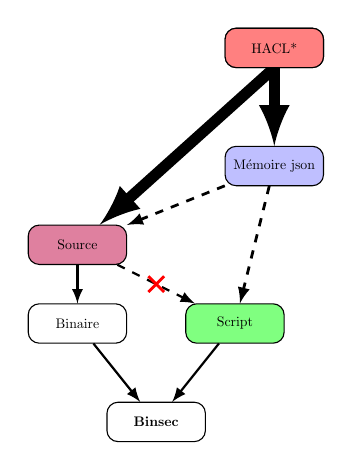
\begin{tikzpicture}[node distance=2cm, scale=0.5, transform shape]
        \tikzset{ block/.style={rectangle,draw,rounded corners,minimum width=2.5cm,minimum height=1cm,align=center},
                arrow/.style={-latex, thick}}
        \node[block] (bin) {Binaire};
        \node[block,  fill=purple!50, above of = bin] (source) {Source};
        \node[block, right of = bin, xshift=2cm, fill=green!50] (src) {Script};
        \node[block, below of = bin, yshift=-0.5cm, xshift=2cm] (binsec) {\textbf{Binsec}};
        
        % Flèches
        \draw[arrow] (bin) -- (binsec);
        \draw[arrow] (src) -- (binsec);
        \draw[arrow] (source) -- (bin);
        \draw[arrow, dashed] (source) -- (src);
        
        \onslide<1>{
            \node[above of = source, xshift=5cm] (json) {};
                \node[block,  fill=red!50, above of = json, yshift=1cm] (hacl) {HACL*};
                \draw[arrow,  line width=4pt] (hacl.south) -- (source);

        };

        \onslide<2>{
        \path (source) -- (src) node[midway] {
            \tikz{\draw[line width=2pt, red] (-0.2,-0.2) -- (0.2,0.2)
                                 (-0.2,0.2) -- (0.2,-0.2);}
        };

        \node[block,  fill=blue!50!white!50, above of = source, xshift=5cm] (json) {Mémoire json};
        \node[block,  fill=red!50, above of = json, yshift=1cm] (hacl) {HACL*};
        \draw[arrow,  line width=1pt, dashed] (json) -- (source);
        \draw[arrow,  line width=1pt, dashed] (json) -- (src);
        \draw[arrow,  line width=4pt] (hacl) -- (json);
        }
    \end{tikzpicture}
  \end{column}
\end{columns}
\end{frame}



\begin{frame}{Fin de stage}
    \begin{columns}
        \begin{column}{0.4\textwidth}
            \begin{blockSimple}{Liste des freins au temps constant}
                \begin{itemize}
                    \item Mécanisme de Pipeline
                    \item Micro instructions
                    \item Renommage des registres
                    \item Prédiction de branches
                    \item Éxecution désordonnée
                    \item In silicium JIT
                \end{itemize}
            \end{blockSimple}
        \end{column}
        \begin{column}{0.6\textwidth}
            \includegraphics[width=\textwidth]{img/pornin.png}
        \end{column}
    \end{columns}
\end{frame}

\end{document}

